\documentclass[border=0pt]{standalone}
\usepackage{fontspec}
% Tinos is used when installed; the fallback keeps this source reproducible.
\IfFontExistsTF{Tinos}{\setmainfont{Tinos}}{\setmainfont{Liberation Serif}}
\usepackage{tikz}
\pagestyle{empty}

\begin{document}
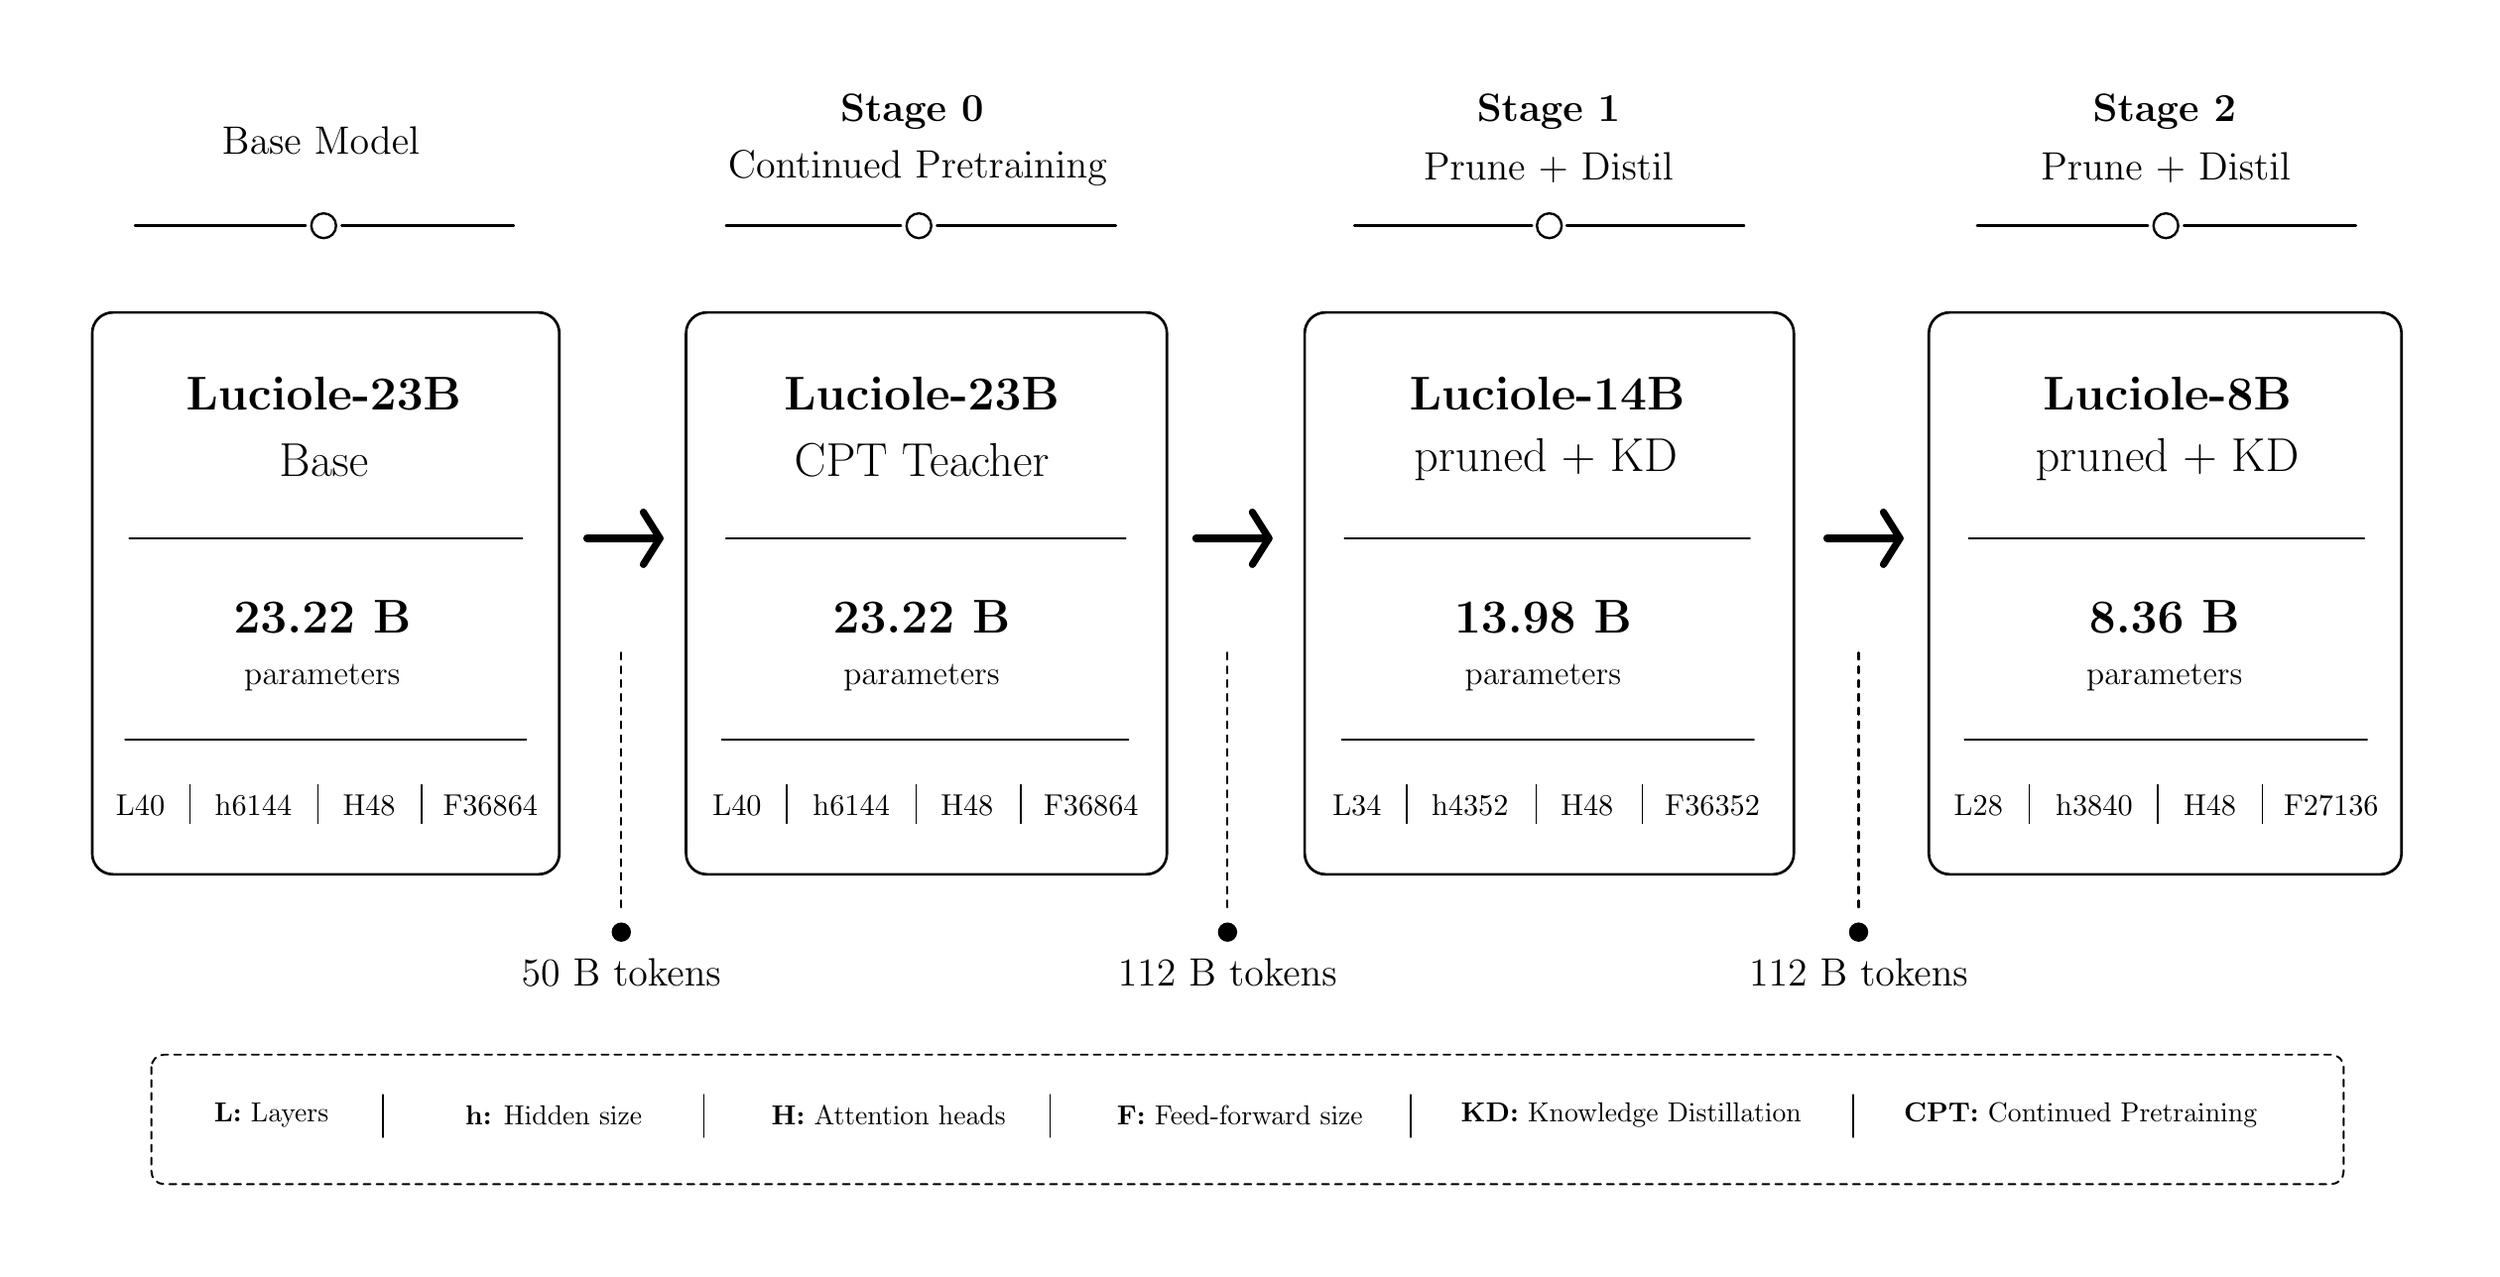
\begin{tikzpicture}[x=0.5bp,y=-0.5bp,line cap=round,line join=round]
  % 1774 x 887 source-image coordinate system; 2 px = 1 bp.
  \path[use as bounding box] (0,0) rectangle (1774,887);

  \tikzset{
    stage/.style={font=\fontsize{14.2bp}{16bp}\selectfont\bfseries,inner sep=0pt,outer sep=0pt},
    subtitle/.style={font=\fontsize{13.2bp}{15bp}\selectfont,inner sep=0pt,outer sep=0pt},
    model/.style={font=\fontsize{16.9bp}{19bp}\selectfont\bfseries,align=center,inner sep=0pt,outer sep=0pt},
    modelsub/.style={font=\fontsize{16.0bp}{18bp}\selectfont,align=center,inner sep=0pt,outer sep=0pt},
    pnum/.style={font=\fontsize{17.7bp}{20bp}\selectfont\bfseries,inner sep=0pt,outer sep=0pt},
    pword/.style={font=\fontsize{12.8bp}{15bp}\selectfont,inner sep=0pt,outer sep=0pt},
    arch/.style={font=\fontsize{10.7bp}{12.5bp}\selectfont,inner sep=0pt,outer sep=0pt},
    token/.style={font=\fontsize{14.0bp}{16bp}\selectfont,inner sep=0pt,outer sep=0pt},
    legend/.style={font=\fontsize{10.4bp}{12bp}\selectfont,inner sep=0pt,outer sep=0pt},
  }

  % Unnumbered base model
  \node[subtitle] at (213,82) {Base Model};
  \draw[line width=0.85bp] (78,144) -- (202,144);
  \draw[line width=0.85bp] (228,144) -- (353,144);
  \draw[line width=0.85bp,fill=white] (215,144) circle[radius=9];

  % Stage 0
  \node[stage] at (642,61) {Stage 0};
  \node[subtitle] at (646,102) {Continued Pretraining};
  \draw[line width=0.85bp] (507,144) -- (634,144);
  \draw[line width=0.85bp] (660,144) -- (790,144);
  \draw[line width=0.85bp,fill=white] (647,144) circle[radius=9];

  % Stage 1
  \node[stage] at (1104,61) {Stage 1};
  \node[subtitle] at (1104,102) {Prune + Distil};
  \draw[line width=0.85bp] (963,144) -- (1092,144);
  \draw[line width=0.85bp] (1117,144) -- (1246,144);
  \draw[line width=0.85bp,fill=white] (1104.5,144) circle[radius=9];

  % Stage 2
  \node[stage] at (1551,61) {Stage 2};
  \node[subtitle] at (1552,102) {Prune + Distil};
  \draw[line width=0.85bp] (1415,144) -- (1539,144);
  \draw[line width=0.85bp] (1565,144) -- (1690,144);
  \draw[line width=0.85bp,fill=white] (1552,144) circle[radius=9];

  % Main cards
  \draw[line width=0.95bp,rounded corners=7.5bp] (47,207) rectangle (386,615);
  \draw[line width=0.95bp,rounded corners=7.5bp] (478,207) rectangle (827,615);
  \draw[line width=0.95bp,rounded corners=7.5bp] (927,207) rectangle (1282,615);
  \draw[line width=0.95bp,rounded corners=7.5bp] (1380,207) rectangle (1723,615);

  % Card 1 text
  \node[model] at (215,266) {Luciole-23B};
  \node[modelsub] at (215,314) {Base};
  \draw[line width=0.75bp] (74,371) -- (359,371);
  \node[pnum] at (214,428) {23.22 B};
  \node[pword] at (214,472) {parameters};
  \draw[line width=0.75bp] (71,517) -- (362,517);
  \node[arch] at (82,565) {L40};
  \draw[line width=0.55bp] (118,550) -- (118,578);
  \node[arch] at (164,565) {h6144};
  \draw[line width=0.55bp] (211,550) -- (211,578);
  \node[arch] at (248,565) {H48};
  \draw[line width=0.55bp] (286,550) -- (286,578);
  \node[arch] at (336,565) {F36864};

  % Card 2 text
  \node[model] at (649,266) {Luciole-23B};
  \node[modelsub] at (649,314) {CPT Teacher};
  \draw[line width=0.75bp] (507,371) -- (797,371);
  \node[pnum] at (649,428) {23.22 B};
  \node[pword] at (649,472) {parameters};
  \draw[line width=0.75bp] (504,517) -- (799,517);
  \node[arch] at (515,565) {L40};
  \draw[line width=0.55bp] (551,550) -- (551,578);
  \node[arch] at (598,565) {h6144};
  \draw[line width=0.55bp] (645,550) -- (645,578);
  \node[arch] at (682,565) {H48};
  \draw[line width=0.55bp] (721,550) -- (721,578);
  \node[arch] at (772,565) {F36864};

  % Card 3 text
  \node[model] at (1103,266) {Luciole-14B};
  \node[modelsub] at (1102,314) {pruned + KD};
  \draw[line width=0.75bp] (956,371) -- (1250,371);
  \node[pnum] at (1100,428) {13.98 B};
  \node[pword] at (1100,472) {parameters};
  \draw[line width=0.75bp] (954,517) -- (1253,517);
  \node[arch] at (965,565) {L34};
  \draw[line width=0.55bp] (1001,550) -- (1001,578);
  \node[arch] at (1047,565) {h4352};
  \draw[line width=0.55bp] (1095,550) -- (1095,578);
  \node[arch] at (1132,565) {H48};
  \draw[line width=0.55bp] (1172,550) -- (1172,578);
  \node[arch] at (1223,565) {F36352};

  % Card 4 text
  \node[model] at (1553,266) {Luciole-8B};
  \node[modelsub] at (1553,314) {pruned + KD};
  \draw[line width=0.75bp] (1409,371) -- (1696,371);
  \node[pnum] at (1551,428) {8.36 B};
  \node[pword] at (1551,472) {parameters};
  \draw[line width=0.75bp] (1406,517) -- (1698,517);
  \node[arch] at (1416,565) {L28};
  \draw[line width=0.55bp] (1453,550) -- (1453,578);
  \node[arch] at (1500,565) {h3840};
  \draw[line width=0.55bp] (1546,550) -- (1546,578);
  \node[arch] at (1584,565) {H48};
  \draw[line width=0.55bp] (1622,550) -- (1622,578);
  \node[arch] at (1672,565) {F27136};

  % Thick open-chevron transition arrows (matching source)
  \foreach \xa/\xt/\xb in {406/447/459,848/889/901,1306/1347/1359}{
    \draw[line width=2.6bp] (\xa,371) -- (\xb,371);
    \draw[line width=2.6bp] (\xt,352) -- (\xb,371) -- (\xt,390);
  }

  % Token annotations
  \foreach \x/\lab in {431/{50 B tokens},871/{112 B tokens},1329/{112 B tokens}}{
    \draw[line width=0.75bp,dash pattern=on 2.5bp off 2.5bp] (\x,454) -- (\x,644);
    \fill (\x,657) circle[radius=7];
    \node[token] at (\x,686) {\lab};
  }

  % Legend
  \draw[line width=0.7bp,rounded corners=4.5bp,dash pattern=on 2.5bp off 2.2bp] (90,746) rectangle (1681,840);
  \node[legend] at (177,790) {\textbf{L:} Layers};
  \draw[line width=0.45bp] (258,775) -- (258,806);
  \node[legend] at (382,790) {\textbf{h:} Hidden size};
  \draw[line width=0.45bp] (491,775) -- (491,806);
  \node[legend] at (625,790) {\textbf{H:} Attention heads};
  \draw[line width=0.45bp] (742,775) -- (742,806);
  \node[legend] at (880,790) {\textbf{F:} Feed-forward size};
  \draw[line width=0.45bp] (1004,775) -- (1004,806);
  \node[legend] at (1164,790) {\textbf{KD:} Knowledge Distillation};
  \draw[line width=0.45bp] (1325,775) -- (1325,806);
  \node[legend] at (1490,790) {\textbf{CPT:} Continued Pretraining};
\end{tikzpicture}
\end{document}
